\documentclass{article}


\usepackage[margin=1in]{geometry}
\usepackage{microtype}
\usepackage[utf8]{inputenc}
\usepackage[T1]{fontenc}
\usepackage{amsmath}
\usepackage{amssymb}
\usepackage{tikz}
\usetikzlibrary{arrows}
\usepackage[printwatermark]{xwatermark}
\newcommand{\floor}[1]{\ensuremath{\left\lfloor #1\right\rfloor}}

%\newwatermark[allpages,color=blue!10,angle=45,scale=1.6,xpos=0,ypos=0]{DRAFT-Joseph Tabadero}
%\usepackage{xcolor}
%\usepackage{graphicx}

\newenvironment{solution}{\paragraph{Solution:}}{\hfill$\blacksquare$}



\newcommand{\abs}[1]{\ensuremath{\lvert #1\rvert}}
\newcommand{\degre}{\ensuremath{^\circ}}

\usetikzlibrary{positioning, decorations}
\makeatletter
\tikzset{
	distance from start/.code={%
		\pgfgetpath\currentpath\pgfprocessround{\currentpath}{\currentpath}%
		\pgf@decorate@parsesoftpath{\currentpath}{\currentpath}%
		\pgfmathparse{#1/\pgf@decorate@totalpathlength}\tikzset{pos=\pgfmathresult}},
	distance from end/.code={%
		\pgfgetpath\currentpath\pgfprocessround{\currentpath}{\currentpath}%
		\pgf@decorate@parsesoftpath{\currentpath}{\currentpath}%
		\pgfmathparse{1-(#1/\pgf@decorate@totalpathlength)}\tikzset{pos=\pgfmathresult}}
}

\title{Solutions to Part II of 18th PMO (Qualifying Stage)}
\author{Joseph S. Tabadero, Jr.}
\date{\today}



\begin{document}
	\maketitle
	
	
	\section*{Part II}
	
	\begin{enumerate}
		\item A married couple has PhP 50, 000 in their joint account. In anticipation of their upcoming
		anniversary, they agreed to split-up evenly and buy each one a gift. However, they agreed
		that they must have enough money left such that when combined, a minimum bank balance
		of PhP 5, 000 is maintained. If the couple individually bought gifts without regard to how
		much the other’s gift will cost and each gift is randomly priced between PhP 0 to PhP
		25, 000, what is the probability that they will be able to maintain the minimum required
		balance after buying the gifts?
		
		
		\begin{solution}
			Let $x$ be the money left with the husband, and $y$ be the money left with the wife after buying their presents. The sample space is $\Omega = [0,25000]\times [0,25000]$. We need to find the probability of the event $\{(x,y)\in \omega: x+y > 5000\}$. Looking at the figure below, we can see that the desired probability is the ratio of the shaded region over the whole rectangular region $\Omega$.
			
			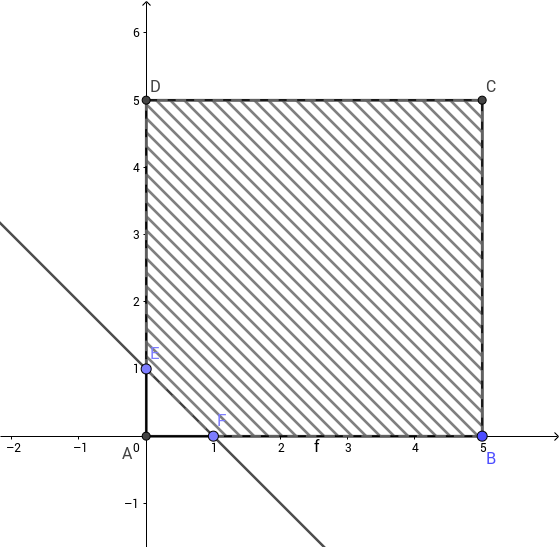
\includegraphics[width=0.6\linewidth]{part3_1}
			
			The desired probability is $1-\dfrac{2500^2}{50000^2}=0.98$. (D)
		\end{solution}
	
	\item What is the difference between the largest and smallest real zeros of the function $f(x)=2x^4-7x^3 + 2x^2 + 7x + 2?$
	
	\begin{solution}
		$f(x)=2x^4-7x^3 + 2x^2 + 7x + 2=(x-2)(2x+1)(x^2-2x-1)=0$.
		The solution set is $\{-\frac{1}{2}, 2, 1\pm \sqrt{2} \}$. Therefore, the difference between the maximum and minimum solutions is $\frac{5}{2}+\sqrt{2}$. (D)
	\end{solution}

	\item Let $S$ be the set of all points A on the circle $x^2 + (y -2)^2 = 1$ so that the tangent line at
	A has a non-negative $y$-intercept; then $S$ is the union of one or more circular arcs. Find
	the total length of $S$.
	
	\begin{solution}
		We note that if the tangent line is along the top semi-circle, its $y$-intercept is always non-negative. That portion of the arc has length $\frac{\pi}{2}$. Now consider the lower semi-circle. We are after the portion between point $A$ and its corresponding point in the second quadrant. To get the coordinates of $A$, we get the solution set of the equations $y=mx$ and the circle  $x^2 + (y -2)^2 = 1$, where $m$ is the slope of the line. We note that $b=0$ in this case. Solving the system for $x$, we get
		\begin{equation}
			x = \frac{4m\pm \sqrt{4m^2-12}}{2(m^2+1)}.
		\end{equation}
		$x$ is unique if $m=\pm\sqrt{3}$. The points of intersection are therefore $(\frac{3}{2}, \frac{3}{2})$ and $(-\frac{\sqrt{3}}{2}, \frac{3}{2})$. To get the angles, we simply translate the center $(0,2)$ to $(0,0)$. The translation gives the coordinates $(\frac{3}{2}, -\frac{1}{2})$ and $(-\frac{3}{2}, -\frac{1}{2})$ with corresponding angles $7\pi/6$ and $11\pi/6$. The length between these angles is $2\pi/3$. $S$ therefore has a length of $\pi + 2\pi/3=5\pi/3$. (B)
		
		
		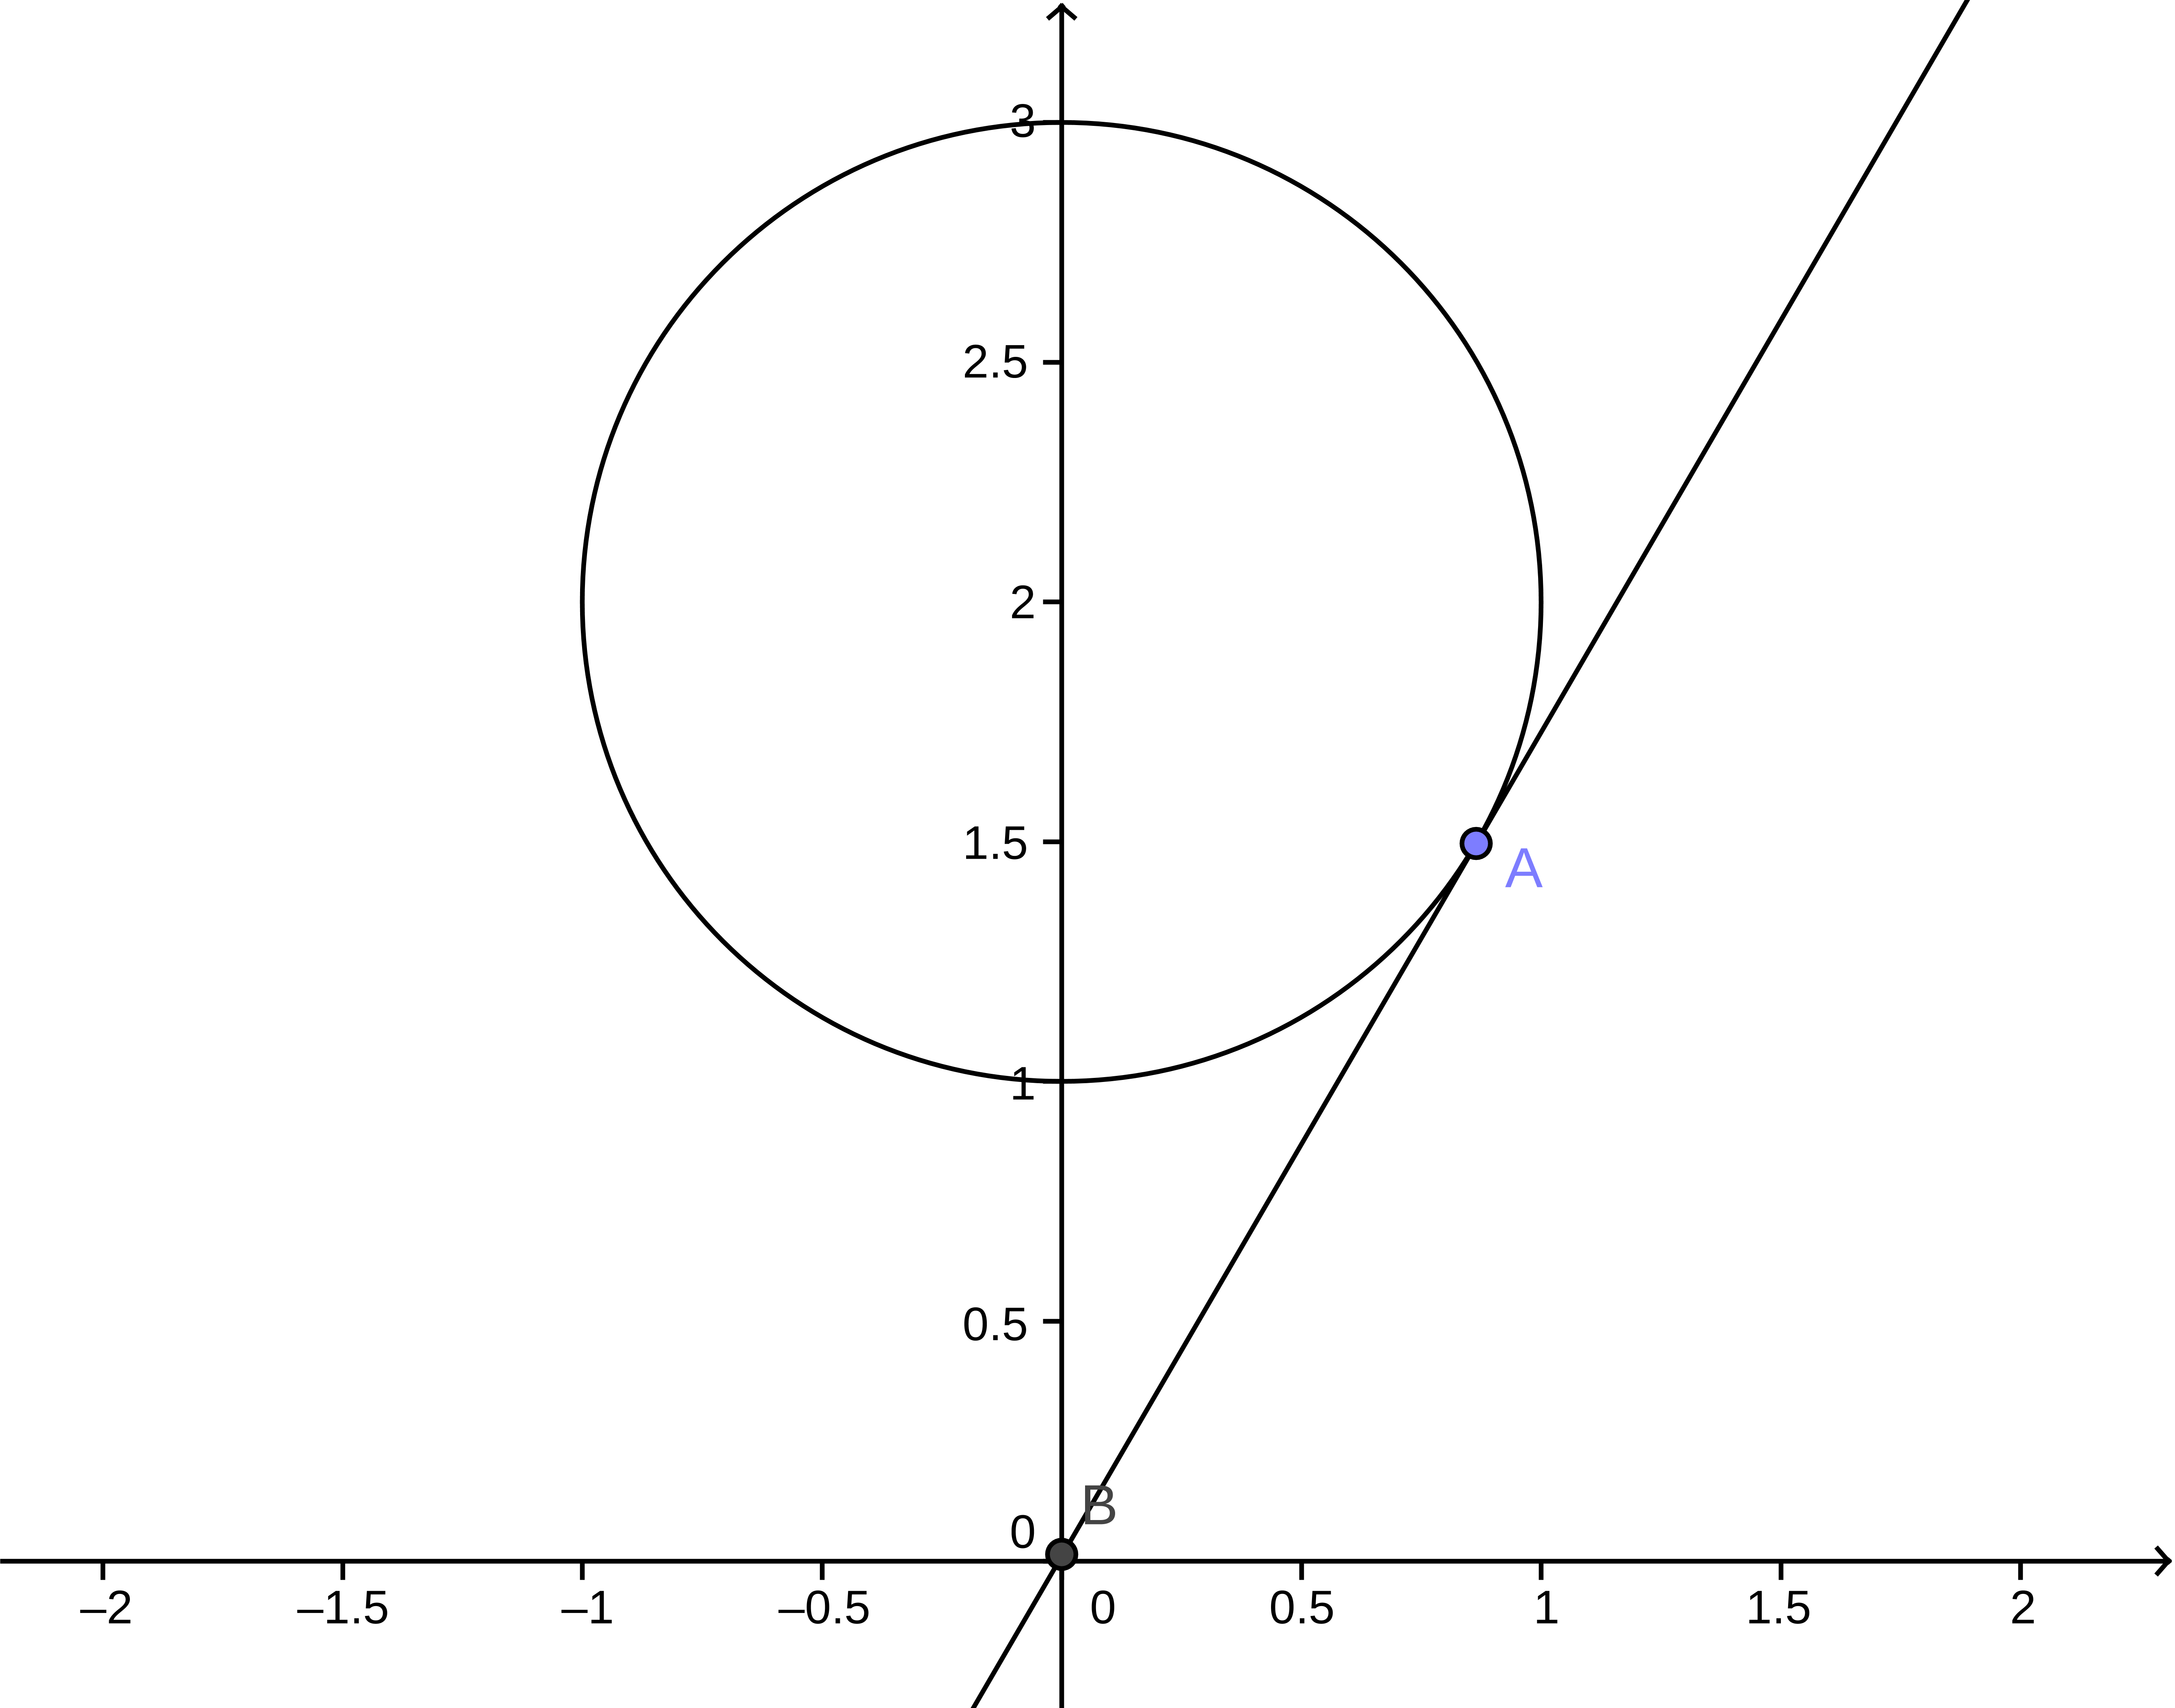
\includegraphics[width=0.7\linewidth]{part2_3}
	\end{solution}

	\item How many positive integers n make the expression $7^n + 7^3 + 2\cdot7^2$ a perfect square?
	
	\begin{solution}
		\begin{equation}
			7^n + 7^3 + 2\cdot 7^2 = 7^2(7^{n-2}+9)=7^2\cdot 4^2
		\end{equation}
		if $n=3$. There are no other values of $n$ for which the given expression is a square. (B)
	\end{solution}

	\item The numbers $1, 2,\ldots , 12$ have been arranged in a circle. In how many ways can five numbers
	be chosen from this arrangement so that no two adjacent numbers are selected?
	
	\begin{solution}
		WLOG, say we arranged the numbers in ascending order. Start at 1, skip 2, choose 3, skip 4, choose 5, skip 6, choose 7. The fifth number can then be one of 9, 10, and 11. We can do this process 12 times. And for each starting number, there are 3 ways of choosing the fifth number. Therefore, there are 36 ways to do the selection. (B)
	\end{solution}

	\item How many (nonconstant) polynomial factors with leading coefficient 1, with the other
	coefficients possibly complex, does $x^2015 + 18$ have?
	
	\begin{solution}
		No idea pa.
	\end{solution}

	\item Let $a = 25^{12}$ , $b = 16^{14}$ , and $c = 11^{16}$ . Which of the following is true?
	
	\begin{solution}
		$c < a < b$. (C)
	\end{solution}

	\item How many integers $x$ are there, where $100 \leq x \leq 2015$, and $x$ is divisible by 3 or 8, but
	not by 6?
	
	\begin{solution}
		There are 671 numbers divisible by 3 between 1 and 2015 and 33 divisible by 3 between 1 and 100. That is, there are 671-33=538 divisible by 3 between 100 and 2015. There are $251-12=139$ divisible by 8, and there are $84-4=80$ divisible by 24. Therefore, of those divisible by 8, there are $139-80=59$ not divisible by 6. Using inclusion-exclusion principle, there are $538+139-80=597$ that are divisible by 8 or 3. Therefore, there are $538-59=479$ divisible by 3 or 8 but not by 6.
	\end{solution}

	\item Find the 2015th digit in 122333444455555...
	
	\begin{solution}
		Use listing to get 5. (B)
	\end{solution}
	
	\item Find the sum of $\displaystyle \sum_{i=1}^{2015}\left\lfloor \frac{\sqrt{i}}{10}\right\rfloor$.
	
	\begin{solution}
		\begin{equation}
		\floor{\frac{\sqrt{i}}{10}} =
			\begin{cases}
			 1 & \text{for}\quad i=1,..., 399\\
			 2 & \text{for}\quad i=400,..., 899\\
			 3 & \text{for}\quad i=900,..., 1599\\
			 4 & \text{for}\quad i=1600,..., 2015\\
			\end{cases}
		\end{equation}
		Therefore, the sum is $300\times 1+ 500\times 2+700\times3 + 416\times 4=5064$.
	\end{solution}
	\end{enumerate}
	
	
\end{document}